
\section{Circuitos integradores y derivadores}
\subsection{Introducción}
Los circuitos implementados con amplificadores operacionales permiten la implementación de diferentes configuraciones que resuelven problemas matemáticos. Con el diseño adecuado pueden usarse para resolver sistemas de ecuaciones diferenciales.
En este caso estudiaremos 2 bloques fundamentales. El circuito integrador y el derivador. Se analizaran sus características más relevantes así como también sus límites de uso y como extenderlos para aprovecharlos al máximo.

\begin{figure}[hbt!]
	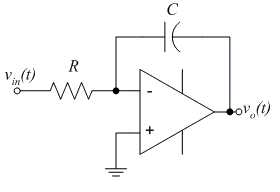
\includegraphics[scale=1]{Ejercicio4/integrador.png}
	\caption{Circuito integrador} 
	
	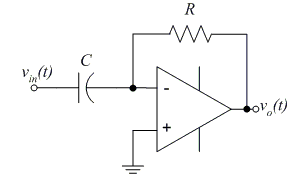
\includegraphics{Ejercicio4/derivador}
	\caption{Circuito Derivador} 
	
\end{figure}

\subsection{Análisis previo del \textbf{LM833N}}
El amplificador a utilizar es el \textbf{LM833N} de STMicroelectronics. El mismo es un operacional de bajo ruido diseñado para aplicaciones relacionadas al manejo de audio.
En su hoja de datos podemos ver que posee un alto nivel Slew Rate de hasta 7 $\frac{V}{s}$, un GBP de 15MHz y una ganancia de tensión 
a lazo abierto típica de unos 110 dB. Notemos que también se indica que la ganancia mínima es de unos 90 dB. 


 \subsubsection{Cálculo de $A_{vol}$}
Para poder realizar los cálculos de transferencia y establecer sus correspondientes transferencias de teóricas primero debemos conocer $A_{vol}$ medido en veces. Para esto basta con tomar el valor de ganancia de tensión típica a veces.
$$A_{vol} = 10^{\frac{110}{20}}$$
$$A_{vol} \approx 316.227,77$$

\subsubsection{Cálculo de  la $f_p$, polo dominante}

Dado el \textbf{GBP} de 15MHz podemos fácilmente calcular la frecuencia de corte a lazo abierto

$$ f_p = \frac{15MHz}{A_{vol}} $$
$$ f_p \approx 47.44Hz$$

\section{Ganancia bajo diferentes condiciones de $A_{vol}$}
En esta sección analizaremos las características de la ganancia de tensión brindad por ambos circuitos bajo diferentes condiciones.

\subsection{$A_{vol}$ infinito}
En un circuito con amplificadores operacionales es deseable utilizar dispositivos con $A_{vol}$(ganancia a lazo abierto) lo más alto posible para que los modelos teóricos se aproximen a su implementación física.

Ambos circuitos adoptan la configuración de un circuito inversor y sus transferencias pueden ser descritas mediante
$$H(s)_{inv} = \frac{-\frac{Z_{Feed}}{Z_{in}}}
{1+\frac{1+\frac{Z_{Feed}}{Z_{in}}}{A_{vol}}} $$
La cual representa la función transferencia de un amplificador operacional no ideal.
Si consideramos $A_{vol}$ infinito obtenemos la transferencia para el inversor ideal:
$$H(s)_{inv} = \frac{-\frac{Z_{Feed}}{Z_{in}}}
				{1+\underbrace{\frac{1+\frac{Z_{Feed}}{Z_{in}}}{A_{vol}}}_{\text{\shortstack{$A_{vol}\rightarrow \infty$ \\ $\rightarrow 0$}}}}$$

$$H(s)_{ideal} =  -\frac{Z_{Feed}}{Z_{in}}$$

Entonces para el circuito integrador obtenemos:
$$H(s)_{\int_{}{}} = \frac{-1}{sCR} $$

Podemos corroborar que la acción de este circuito es integrar la señal de entrada al realizar la transformada inversa de Laplace
$$v_{out}(t) = \mathcal{L}^{-1}[X(s)H(s)_{\int_{}{}}]$$
$$v_{out}(t) = \mathcal{L}^{-1}[X(s)\cdot \frac{-1}{sCR}]$$
$$v_{out}(t)= \frac{-1}{CR} \cdot \int_{0}^{t}v_t dt$$            
\\
Por otro lado tenemos el circuito derivador:
$$H(s)_{\frac{d}{dt}}=-sCR$$
Análogamente aplicamos la anti-transformada de Laplace:

$$v_{out}(t) = \mathcal{L}^{-1}[X(s)H(s)_{\frac{d}{dt}}]$$

$$v_{out}(t) = \mathcal{L}^{-1}[X(s)\cdot (-sCR)]$$

$$v_{out}(t)= -CR \frac{d}{dt}v_t(t)$$       

Si bien, estos circuitos tienen la capacidad de realizar las operaciones antes mencionadas, en los párrafos siguientes estudiaremos su comportamiento y bajo que condiciones funcionan.

\subsubsection{Diagramas de Bode con $A_{vol}$ ideal}
\begin{figure}[H]
	\centering
	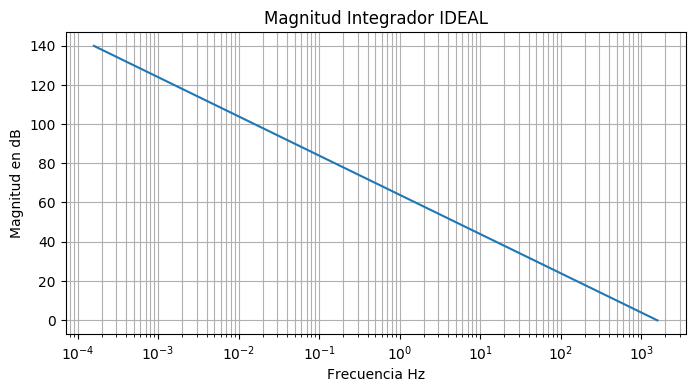
\includegraphics[width=\textwidth]{Ejercicio4/BODE-IDEAL-MAGNITUD-INTEGRADOR.png}
	\caption{Ganancia Ideal Circuito Integrador}
\end{figure}

Observamos que el integrador ideal tiene una muy alta ganancia a bajas frecuencias y muy baja cuando se acerca a los $10KHz$ lo cual limita su rango de operación.

\begin{figure}[H]
	\centering
	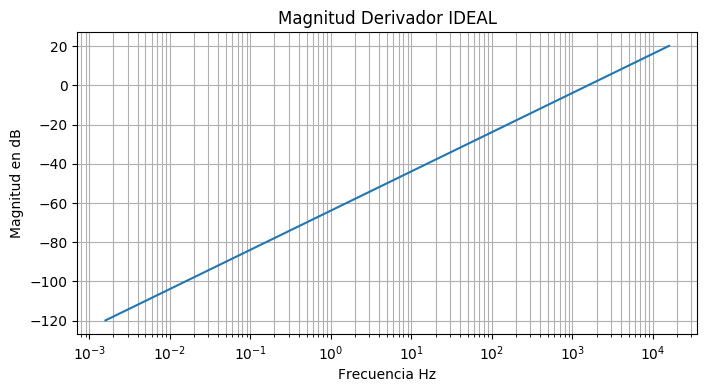
\includegraphics[width=\textwidth]{Ejercicio4/BODE-IDEAL-MAGNITUD-DERIVADOR.png}
	\caption{Ganancia Ideal Circuito Derivador}
\end{figure}
De modo contrario el derivador exhibe sus capacidades a altas frecuencias
\\*
En cuanto a la fase en ambos casos podemos observar como ver cómo las operaciones de integración y diferenciación introducen un desfase de $\pm90^{\circ}$ de la señal original según el caso. 
\begin{figure}[H]
	\centering
	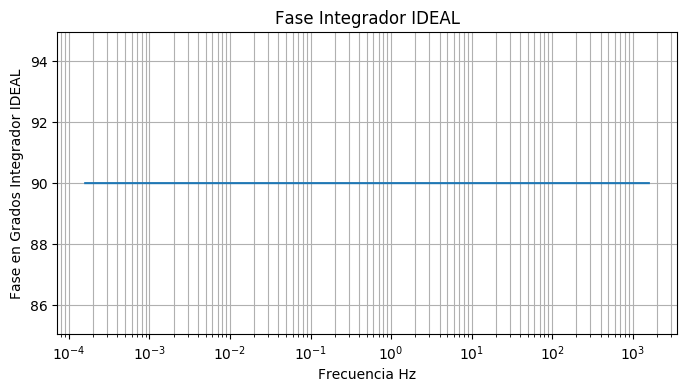
\includegraphics[width=\textwidth]{Ejercicio4/BODE-IDEAL-FASE-INTEGRADOR.png}
	\caption{Fase Ideal Circuito Integrador}
\end{figure}

\begin{figure}[H]
	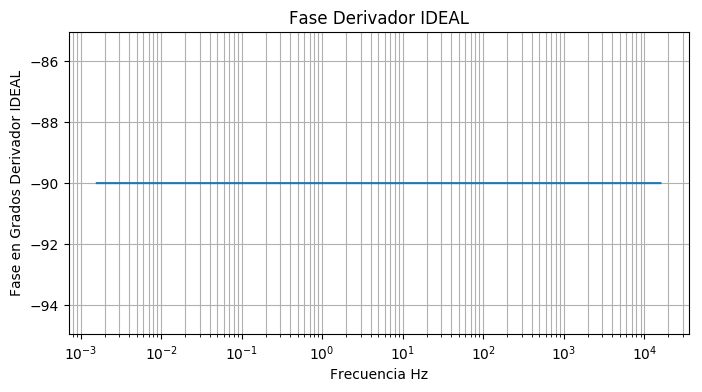
\includegraphics[width=\textwidth]{Ejercicio4/BODE-IDEAL-FASE-DERIVADOR.png}
	\caption{Fase Ideal Circuito Derivador}
\end{figure}

\subsection{$A_{vol}$ finito}
La ganancia a lazo abierto nunca es infinita en los amplificadores operacionales aunque por cuestiones de simplicidad podemos tratarlo como así fuese. En la introducción calculamos el $A_{vol}$ del \textbf{LM833} a partir de los datos brindados por el fabricante en la hoja de datos y encontramos que este valor se encuentra aproximadamente en $31.6227,77$.
Ahora podemos volver a mirar a la función transferencia del inversor no ideal presentada al comienzo.
$$H(s)_{inv} = \frac{-\frac{Z_{Feed}}{Z_{in}}}
{1+\frac{1+\frac{Z_{Feed}}{Z_{in}}}{A_{vol}}} $$

AÑADIR TRANSFERENCIAS!!

\subsubsection{Diagramas de Bode con $A_{vol}$ finito}
\begin{figure}[H]
	\centering
	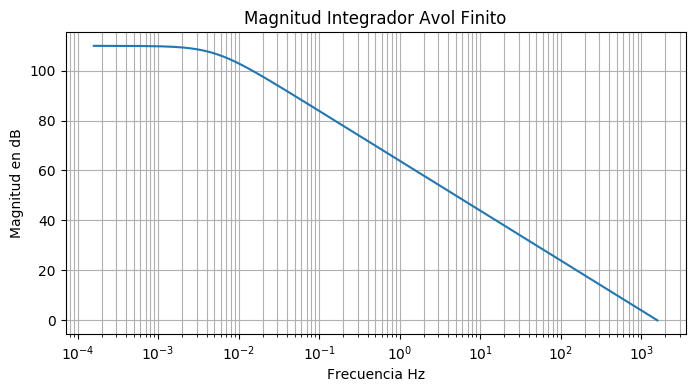
\includegraphics[width=\textwidth]{Ejercicio4/BODE-AVOL-FINITO-MAGNITUD-INTEGRADOR}
	\caption{Ganancia con $A_{vol}$ finito Circuito Integrador}
\end{figure}

\begin{figure}[H]
	\centering
	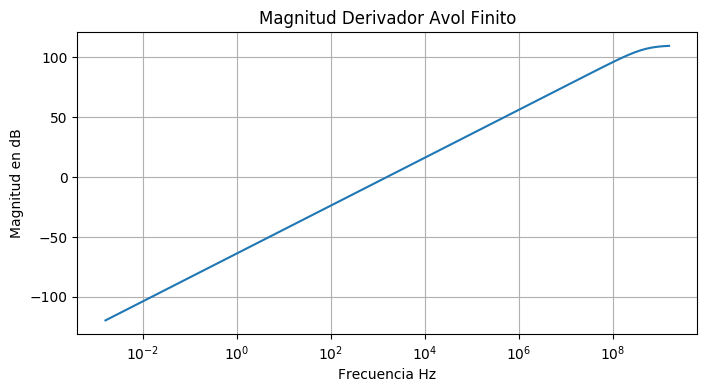
\includegraphics[width=\textwidth]{Ejercicio4/BODE-AVOL-FINITO-MAGNITUD-DERIVADOR}
	\caption{Ganancia con $A_{vol}$ finito Circuito Integrador}
\end{figure}

Al considerar que $A_{vol}$ no tiene un valor infinitamente grande observamos que el circuito integrador se comporta como un filtro pasabajos cuya frecuencia de corte se encuentra a muy baja frecuencia lo cual no permitiría hacer uso del mismo con señales de frecuencia media-alta.
Tambien cabe destacar la gran ganancia que obtienen las señales de baja frecuencia, este es un problema dado que señales parásitas de baja frecuencia consiguen saturar al operacional con facilidad no permitiendo lograr el efecto deseado.

En el caso del derivador ocurre lo contrario, es necesario alcanzar frecuencias en el orden de los $100KHz$ para poder ver una señal sin tanta atenuación. Pero tampoco sera posible y mucho más allá dado que la ganancia brindada rápidamente saturara al opamp lo cual nuevamente limita el rango de operación del circuito. 

\begin{figure}[H]
	\centering
	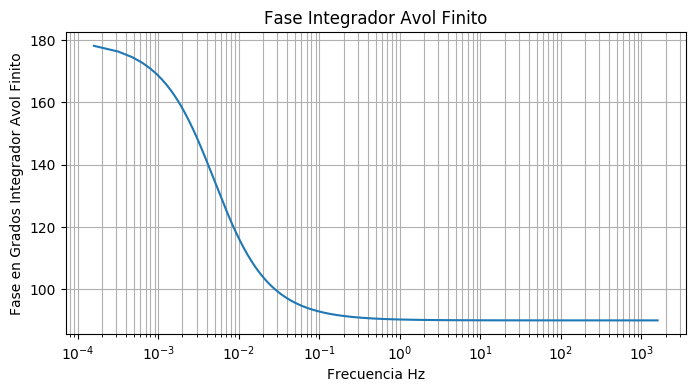
\includegraphics[width=\textwidth]{Ejercicio4/BODE-AVOL-FINITO-FASE-INTEGRADOR}
	\caption{Ganancia con $A_{vol}$ finito Circuito Integrador}
\end{figure}

\begin{figure}[H]
	\centering
	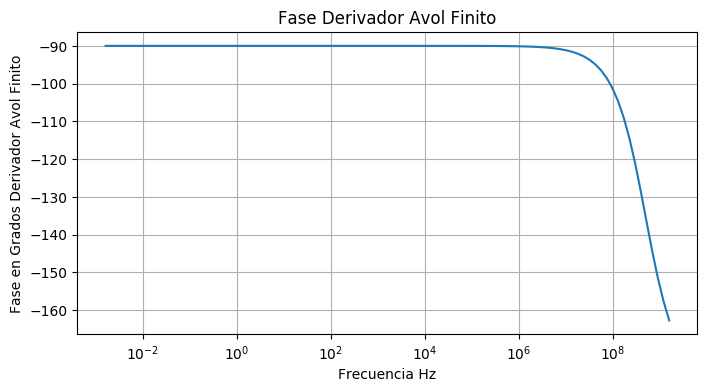
\includegraphics[width=\textwidth]{Ejercicio4/BODE-AVOL-FINITO-FASE-DERIVADOR}
	\caption{Ganancia con $A_{vol}$ finito Circuito Integrador}
\end{figure}

\subsection{Análisis con Polo Dominante}
Con la finalidad de obtener resultados predecibles e independizarse los más posible de las capacidades parasitas del amplificador operacional, los fabricantes añaden el llamado \textbf{polo dominante}. Este polo tiene como finalidad evitar inversiones inesperadas.